\documentclass{beamer}
%
% Choose how your presentation looks.
%
% For more themes, color themes and font themes, see:
% http://deic.uab.es/~iblanes/beamer_gallery/index_by_theme.html
%
\mode<presentation>
{
	\usetheme{Luebeck}      % or try Darmstadt, Madrid, Warsaw, ...
	\usecolortheme{dolphin} % or try albatross, beaver, crane, ...
	\usefonttheme{structuresmallcapsserif}  % or try serif, structurebold, ...
	\setbeamertemplate{navigation symbols}{}
	\setbeamertemplate{caption}[numbered]
} 

\usepackage[english]{babel}
\usepackage[utf8]{inputenc}

\title[ESPN's Total QBR]{Investigation of ESPN's Total Quarterback Rating}
\author{Justin Gomez}
\institute{Montana State University}
\date{April 17, 2017}

\begin{document}
	
	\begin{frame}
		\titlepage
	\end{frame}
	
	% Uncomment these lines for an automatically generated outline.
	%\begin{frame}{Outline}
	%  \tableofcontents
	%\end{frame}
	
	\section{Introduction}
	
	\begin{frame}{Outline}
		\begin{columns}
			\column{0.5\textwidth}
			\begin{itemize}
				\item ESPN's Total QBR
				\item Collected Data
				\item Regression Trees
				\item Bootstrap Aggregation
				\item Gradient Boosting
			\end{itemize}
			\column{0.5\textwidth}
			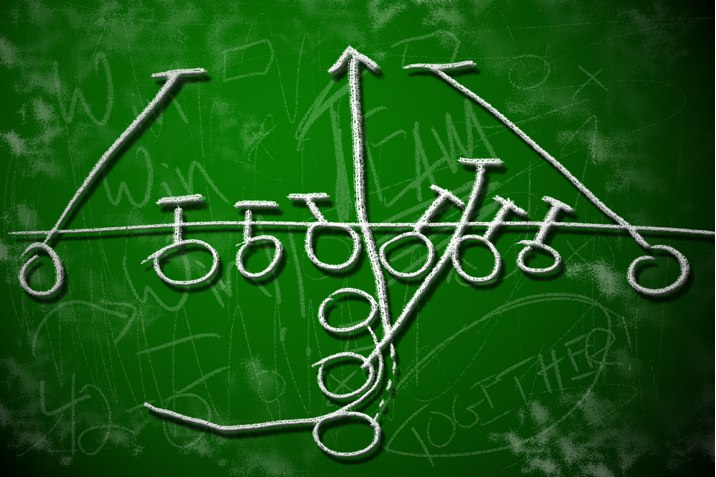
\includegraphics[scale=.2]{football-strategy.jpg}
		\end{columns}
	\end{frame}
	
	\begin{frame}{ESPN's Total QBR}
		\begin{itemize}
			\item Developed in 2011 as a competitor for the NFL's ``passer rating" (which ranges from 0 to 158.3)
			\item Uses play-by-play data
			\item Updates continuously as game plays out
			\item QB must play at least 21 ``action plays"
		\end{itemize}
		\begin{block}{Pros/Cons}
		\begin{columns}
			\begin{column}[t]{0.4\textwidth}
				Pros
				\begin{itemize}
					\item Intuitive scale (0-100)
					\item Utilizes a great deal of information
					\begin{itemize}
						\item Win Probability
						\item Expected Points
						\item Division of Credit
						\item Clutch Index
					\end{itemize}
				\end{itemize}
			\end{column}
			
			\begin{column}[t]{0.5\textwidth}
				Cons
				\begin{itemize}
					\item Complicated
					\item Expensive
					\item Vaguely explained
					\item Subjective
					\item Proprietary
				\end{itemize}
			\end{column}
		\end{columns}
		\end{block}
	\end{frame}

	\begin{frame}{Study Design}
		\begin{itemize}
			\item Initial data set: more than 5000 ratings over 11 years
			\begin{itemize}
				\item Training set: 50\% of initial set
				\item Testing set: 30\% of initial set
				\item Validation set: 20\% of initial set
			\end{itemize}
			\item Fit models on training set
			\item Generate predictions on testing set
			\item After selecting final model, generate predictions on validation set
		\end{itemize}
	\end{frame}

	\begin{frame}{Variables}
				Using post-game summary data rather than play-by-play information, can we accurately predict ESPN's total QBR?
		\begin{itemize}
			\item Seven Predictors:
			\begin{itemize}
				\item Completion Percentage
				\item Number of interceptions
				\item Number of fumbles
				\item Total yards
				\item Game result
				\item Number of sacks
				\item Total touchdowns
			\end{itemize}
		\end{itemize}
	\end{frame}

	%\begin{frame}{Variables and Models}
		%\vspace{-4pt}
		%\begin{columns}
			%\column{\dimexpr\paperwidth-20pt}
			%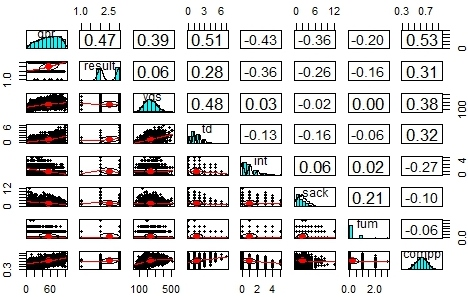
\includegraphics[scale=.95]{variablespanels.jpeg}
		%\end{columns}
	%\end{frame}
	
	\section{Methods}
	
%	\begin{frame}{Methods Overview}
%		Four modeling techniques:
%		\begin{itemize}
%			\item Linear models
%			\item Generalized additive models
%			\item Regression trees
%			\item Random forests
%		\end{itemize}
%		Two improvement algorithms:
%		\begin{itemize}
%			\item Bootstrap Aggregating (bagging)
%			\item Boosting
%		\end{itemize}
%	\end{frame}

	\begin{frame}{Simple Model}
		How well do completion percentage and number of touchdowns predict QBR?
		\begin{columns}
			\begin{column}[t]{.6\textwidth}
				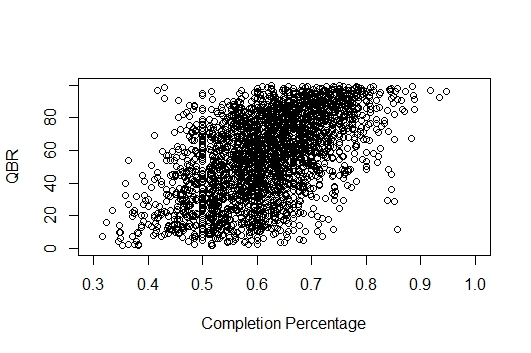
\includegraphics[scale=.45]{scatter1.jpeg}
			\end{column}
			\begin{column}[t]{.6\textwidth}
				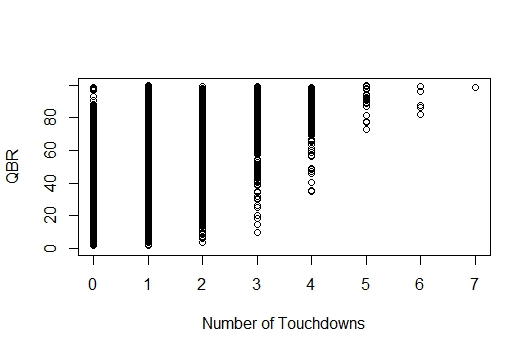
\includegraphics[scale=.28]{scatter2.jpeg}
			\end{column}
		\end{columns}
	\end{frame}

	\begin{frame}{Regression Trees}
		Excellent predicting technique\\
		Primary goal: partitioning the predictor space\\
		\vspace{20pt}
		\begin{columns}
			\begin{column}[t]{0.5\textwidth}
				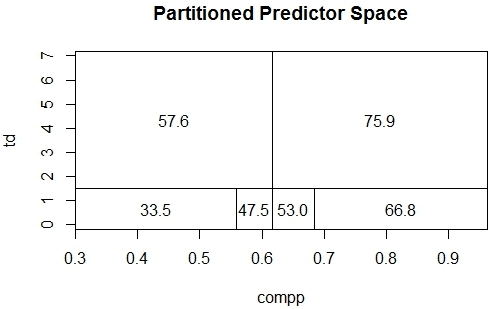
\includegraphics[scale=.45]{expartspace.jpeg}
			\end{column}
			\begin{column}{0.08\textwidth}
			\end{column}
			\begin{column}[t]{\dimexpr\paperwidth-20pt}
				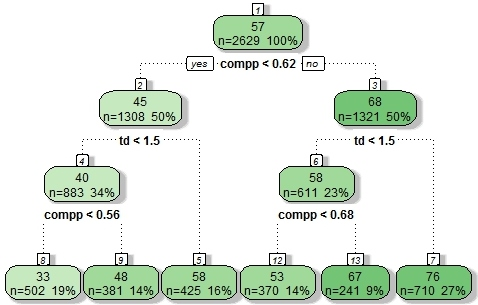
\includegraphics[scale=.5]{extree.jpeg}
			\end{column}
		\end{columns}
	\end{frame}

	\begin{frame}{Bootstrap Aggregation (Bagging)}
		\begin{columns}
			\begin{column}{0.5\textwidth}
				\begin{itemize}
					\item High level algorithm:
					\begin{itemize}
						\item Obtain bootstrap sample
						\item Grow regression tree
						\item Use tree to predict values\\
						for new observations
						\item Repeat many times
						\item Aggregate predictions 
					\end{itemize}
					\item Benefits:
					\begin{itemize}
						\item Prediction variance reduced
						\item More accurate
						\item Helps avoid overfitting
					\end{itemize}
				\end{itemize}
			\end{column}
			\begin{column}{0.5\textwidth}
				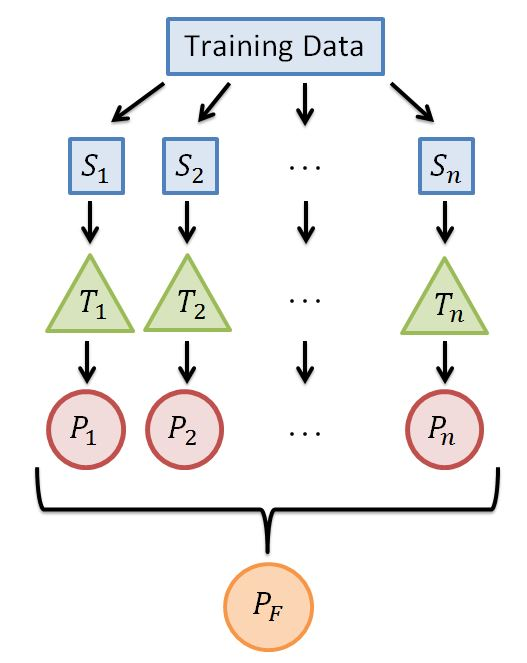
\includegraphics[scale=.4]{baggingalg.jpg}
			\end{column}
		\end{columns}
	\end{frame}

	\begin{frame}{Gradient Boosting}
		\begin{itemize}
			\item High level algorithm:
			\begin{itemize}
				\item Grow tree with training set
				\item Predict values for new observations
				\item Find residuals for predictions
				\item Grow tree with residuals
				\item Repeat many times
			\end{itemize}
			\item Performed on full training set
			\item Slow learning algorithm
			\item Typically results in best predictions
		\end{itemize}
	\end{frame}

	\begin{frame}{Boosting Example}
		\begin{columns}
			\begin{column}{0.5\textwidth}
					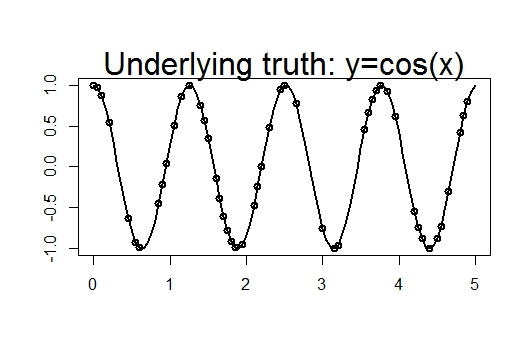
\includegraphics[scale=0.35]{data.jpeg}\\
					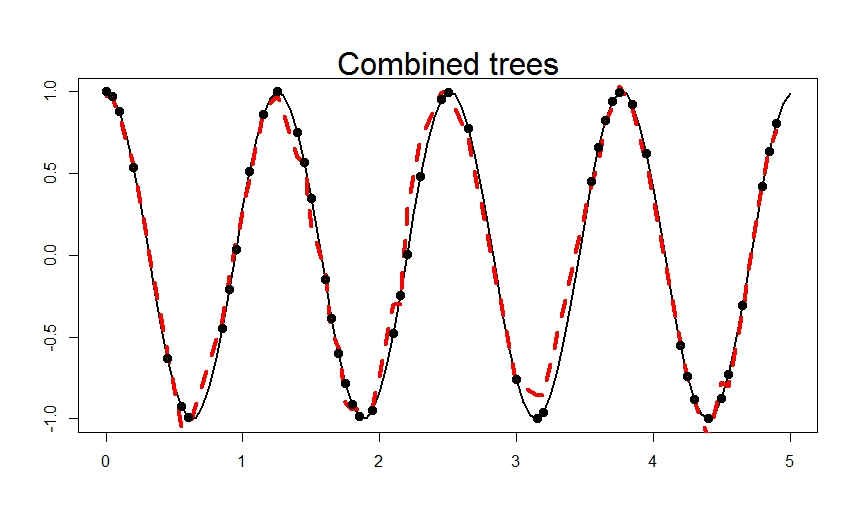
\includegraphics[scale=0.35]{combine.jpeg}\\
			\end{column}
			\begin{column}{0.6\textwidth}
				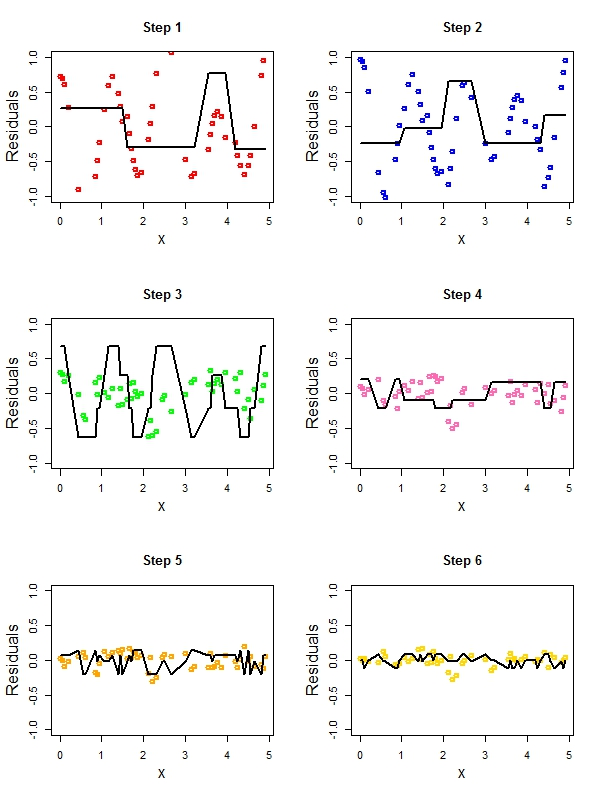
\includegraphics[scale=0.365]{boostex.jpeg}
			\end{column}
		\end{columns}
	\end{frame}
	
	\section{Results}
	
	\begin{frame}{Choosing the Best Performer}
		\begin{itemize}
			\item Models judged and compared according to RMSE
		\end{itemize}
		\begin{equation}
			RMSE=\sqrt{\frac{\sum_{i=1}^{n}(\hat{y_{i}}-y_{i})^{2}}{n}}
		\end{equation}		
		\begin{itemize}
			\item Small RMSE indicates good predictive power
		\end{itemize}
		\begin{table}
			\centering
			\begin{tabular}{|c|c|c|}
				\hline
				Base Tree & Bagged Tree & Boosted Tree\\
				\hline
				21.138 & 20.401 & 19.920\\
				\hline
			\end{tabular}
		\caption{RMSEs for simple model with QBR as the response and completion percentage and touchdowns as predictors.}
		\end{table}
	\end{frame}

	\begin{frame}{Conclusions}
		\begin{itemize}
			\item Trees are powerful tools for prediction
			\item Bagging and boosting offer improved predictions
		\end{itemize}
		Further work:
		\begin{itemize}
			\item Expand model space to more complex models
			\item Fit linear/generalized additive models, random forests
			\item Select best prediction method and generate final RMSE
		\end{itemize}
	\end{frame}

	\begin{frame}{References}
		\begin{itemize}
			\item \textit{NFL Quarterback Rating Formula}. \url{http://www.nfl.com/help/quarterbackratingformula}.
			\item Faraway, J. J. \textit{Linear Models with R}. Taylor and Francis, 2009.
			\item James, G., Witten, D., Hastie, T., and Tibshirani, R. \textit{An Introduction to Statistical Learning}. Springer, 2015.
			\item Kuhn, M., and Johnson, K. \textit{Applied Predictive Modeling}. Springer, 2013. \url{http://bleacherreport.com/articles/1640782-the-anatomy-of-a-53-man-roster-in-the-nfl}, 2013.
			\item Oliver, D. \textit{Guide to the Total Quarterback Rating}.\\
			\url{http://www.espn.com/nfl/story/_/id/6833215/explaining-statistics-total-quarterback-rating}, 2011.
		\end{itemize}
	\end{frame}
	
\end{document}
